\section{Introduction}
\label{sec:introduction}


Fix a field $\K$ and an element $q\neq 1,0\in \K$. Let
$e$ be the multiplicative order of $q$. In this paper, we
discuss isomorphisms between two different families of algebras
constructed from this data.

One of these families is
ultimately descended from Erich Hecke, though it is a rather distant
descent. It's not clear he would recognize these particular progeny.
The other family is of a more recent vintage. While the first hint of
its existence was the nilHecke algebra acting on the cohomology of the
complete flag variety, it was not written in full generality until the
past decade in work of Khovanov, Lauda and Rouquier~\cite{KLI,KLII,Rou2KM}. 

In the spirit of
other families in representation theory, one can think of Hecke family
as being \emph{trigonometric} and the KLR family as \emph{rational}. However, a common phenomenon
in mathematics is the existence of an isomorphism between
trigonometric and rational versions of an object after suitable completion; the
``ur-isomorphism'' of this type is between the associated graded of
the K-theory of a manifold and its cohomology. Such an isomorphism
has been given for completions of non-degenerate and degenerate affine
Hecke algebras by Lusztig in~\cite{Lusgraded}. Another similar
isomorphism is given in~\cite{GTL} for Yangians and quantum affine
algebras. In this paper, we will define isomorphisms with a similar
flavor between the algebras in the Hecke and KLR families. These
isomorphisms are between certain special completions; before
discussing the specific examples, we cover some generalities on this
type of completion in Section~\ref{sec:polyn-style-repr}.

In both cases, these families have somewhat complicated family
trees. Every one depends on a choice of a rank, which we will denote $n$
throughout. In the diagrammatics, this will always correspond to a
number of strands. On the Hecke side, we will always have a dependence
on a parameter $q$, which we will sometimes want to deform to $qe^h$
with a $h$ a formal parameter. On the KLR side, we will not see an
explicit family of algebras as we vary $q$, but the underlying
Dynkin diagram used in the definition of these algebras will depend on $h$. 

Like blood types, there are two complementary ways that they can
become complicated. The simplest case, our analogue of blood type O,
is the affine Hecke algebra (on the Hecke side) and the KLR algebra of
the Dynkin diagrams $\hat{A}_e/A_\infty$ (on the KLR side). The two complications we can
add are like the type A and type B antigens on our red blood cells.
Since ``type A/B'' already have established connotations in
mathematics, we will instead call these types W and F:
\begin{itemize} 
\item algebras with the type W complication are ``weighted''\footnote{The referee has suggested that
 ``wraith'' in reference to the ghost strands which appear might be
 more appropriate. You might very well think that; the author couldn't possibly comment.} : these
 include affine $q$-Schur algebras~\cite{GreenSchur} (on the Hecke side) and weighted KLR
 algebras~\cite{WebwKLR}.
\item algebras with the type F complication are 
 ``framed'': these include cyclotomic Hecke algebras~\cite{AK} and the
 $\hat{A}_e/A_\infty$ tensor product categorifications from
~\cite{Webmerged}. These are analogs of the passage from Lusztig to
 Nakajima quiver varieties.
\item finally, both of these complications can be present
 simultaneously, giving type WF. The natural object which appears in
 the Hecke family is the category $\cO$ of a Cherednik algebra $\Z/e\Z\wr
 S_n$~\cite{GGOR}, though in a guise in which has not been seen previously. On
 the KLR side, the result is a steadied quotient of a weighted KLR
 algebra for the Crawley-Boevey quiver of a dominant weight of type
 $\hat{A}_e/A_\infty$ (see Definition~\ref{def:WF-KLR} and~\cite[\S~3.1]{WebwKLR}).
\end{itemize}

Our main theorem is that in each type, there are completions of these
Hecke- and KLR-type algebras that are isomorphic.

Since a great number of different algebras of representation theoretic
interest appear in this picture, it can be quite difficult to keep
them all straight. For the convenience of the reader, we give a table
in Figure~\ref{table-of-algebras}, placing all the algebras and categories which appear in this picture in their
appropriate type. Note that many of the items listed below (such as
Ariki--Koike algebras, or cyclotomic $q$-Schur and quiver Schur
algebras) are not the most general family members of that type, but
rather special cases. We'll ultimately focus on the category of
representations of a given algebra, so we have not
distinguished between Morita equivalent algebras. 

\begin{figure}[htb]\label{table-of-algebras} \centering
\renewcommand{\arraystretch}{1.4}
 \begin{tabular}{|c|p{43mm}|p{68mm}|} 
 \hline
 Type& KLR side & Hecke side \\
\hline 
O&KLR algebra \gls{R}~\cite{KLI,Rou2KM}
& affine Hecke algebra \gls{mH} of type A (Thm.~\ref{type-O-Hecke})\\ 
\hline
W& weighted KLR algebra~\cite{WebwKLR}, quiver Schur algebra~\cite{SWschur} & 
affine $q$-Schur algebra $\gls{cS}(n,m)$ (Thm.~\ref{waha-Schur})\\ 
\hline
F& cyclotomic KLR algebras~\cite{KLI}, algebras $\gls{cT}$ categorifying tensor products 
for type $A/\hat{A}$~\cite{Webmerged} &
cyclotomic Hecke (Ariki--Koike) algebras (Prop.~\ref{prop:cyclo-Hecke}), 
category $\cO$ for $\mathfrak{gl}_N$ ($e=\infty$) (\cite[9.11]{Webmerged})\\ 
\hline
WF& reduced steadied quotients $\gls{cdalg}^\vartheta$ categorifying Uglov Fock spaces~\cite{WebRou}, cyclotomic quiver Schur algebras~\cite{SWschur}&
 category $\cO$ for a
Cherednik algebra with $\Z/e\Z\wr S_n$ (\cite[Thm.~A]{WebRou}),
cyclotomic $q$-Schur algebras (Prop.~\ref{cqs-morita}) \\ 
\hline
\end{tabular}
\caption{The algebras of interest.}
\end{figure}
 
 
 
On the KLR side, the diagrammatic formulation we give matches the
original definition of these algebras (with the exception of quiver
Schur algebras, which are shown to be Morita equivalent to certain
reduced steadied quotients in~\cite[Th.~3.9]{WebwKLR}). For
the Hecke side, typically our description is a bit different from the
definitions readers will be used to, and we have
listed the result in this paper or another which gives the relation.

\begin{rema}
 All of the algebras on the Hecke side of this list have degenerate
 analogues, and we could have written this paper, like~\cite{BKKL}
 with parallel sets of formulas in the degenerate and non-degenerate
 cases. We avoided doing this because of length, because the correspondence between
 degenerate and non-degenerate formulas is easy to work out (just replace
 multiplication by $q^{\pm 1}$ by addition of $\pm 1$), and our
 ultimate goal is to apply our results to the Cherednik category
 $\cO$ in~\cite{WebRou},
 which only uses the non-degenerate case. 
\end{rema}

\begin{rema}
 Very closely related (and in many cases, Morita equivalent) algebras
 were introduced by Maksimau and Stroppel~\cite{MS18}; they use the
 terms ``Hecke family'' and ``KLR family'' exactly as above. The
 main difference between the approaches in these papers is that this
 paper emphasizes not Schur algebras as those working in the field
 understand them, but certain Morita equivalent algebras we find more
 convenient to work with, whereas~\cite{MS18} work more directly
 with the Schur algebra. 
\end{rema}

\subsubsection*{Type O} We'll first consider the simplest case of
this isomorphism. In essence, this is just a rewriting of the
approach in 
\cite[\S~3.2]{Rou2KM}, but for applications in~\cite{WebRou}, we require
a small generalization of those results, and it will serve to
illustrate our techniques for the sections on other types. The two algebras we consider are:
\begin{itemize}
\item the affine Hecke algebra $\gls{mH}(\pq)$ of
$S_n$ with parameter $qe^h$, considered as a $\K\llbracket h\rrbracket$-algebra. Note
that this deformation only makes sense if $\K$ has characteristic~0.
\item the KLR algebra $\gls{R}(h)$ of rank $n$ for
$\slehat$ attached to the polynomials $Q_{i+1,i}(u,v)=u-v+h$, also
considered over $\K\llbracket h\rrbracket$.
\end{itemize}
These algebras are defined in~\cite[(4.1--5)]{BKKL} and
\cite[(1.6--15)]{BKKL} respectively; here we consider them with
the addition of an $h$-adic deformation. This deformation is very
important since it allows us to compare affine Hecke algebras with $q$
at a root of unity with those for generic $q$. 
For KLR algebras, this
corresponds to comparing KLR algebras for $\widehat{A}_e$ and
$A_\infty$ (as in~\cite[Ex.~2.25]{WebwKLR}).
By the usual idempotent lifting arguments (see, for example,
\cite[Lem.~2.2]{Kbook}), the Grothendieck group of
projective modules for $\gls{R}(h)$ is the same as that for the usual KLR
algebra $R$ with $h$ set to $0$; thus, $\gls{R}(h)$-modules categorify the
algebra $U^+(\mathfrak{sl}_\infty)$ or
$U^+(\mathfrak{\widehat{sl}}_e)$ by~\cite[Thm.~8]{KLII}.

\begin{theorem} \label{thm:O-main}
 There is a $\K\llbracket h\rrbracket $-algebra isomorphism $\hmH(\pq)\cong \hR(h)$. 
\end{theorem}
The characteristic 0 assumption may look peculiar to experts in the
field; the Hecke algebra over a field of characteristic $p$ has
similar deformations coming from deforming the parameter $q$ (though
$e^h$ does not make sense here), but it's not clear how to match other
deformations of the Hecke algebra with the simplest deformations of
the KLR algebra. 
A different deformation of the KLR algebra defined by Hu and Mathas~\cite{HMsemi} is
compatible with more general deformations of the Hecke algebra, in particular with the
deformation of $\mathbb{F}_p[S_n]$ to $\mathbb{Z}_p[S_n]$. 
Since our primary applications will be to Hecke algebras and
related structures of characteristic 0, this hypothesis is no problem
for us. In general, we'll prove our results in parallel with the undeformed Hecke
algebra (and related structures) in arbitrary characteristic, and with
the exponentially deformed Hecke algebra in characteristic 0.

One isomorphism between type O completions was implicitly constructed by Brundan and
Kleshchev in~\cite{BKKL} and for a related localization by Rouquier in
\cite[\S~3.2.5]{Rou2KM} for $h=0$. Unfortunately, it is not clear how
to extend these isomorphisms to the deformed case, so instead we
construct an isomorphism which is different even after the
specialization $h=0$. This isomorphism still has a similar flavor to those previously
defined; in brief, we use a general power series of the form
$1+y+\cdots$ (in particular $e^y$) where Brundan and Kleshchev or
Rouquier use $1+y$. 

We will also generalize this theorem in a small
but useful way: in fact there is a natural class of completions of the Hecke
algebra that correspond with the KLR algebra for a larger Lie
algebra $\mathfrak{G}_{\gls{U}}$. Here we consider an arbitrary finite subset $\gls{U}\subset \K\setminus\{0\}$, given a graph
structure connecting $u$ and $u'$ if $qu=u'$, and let $\mathfrak{G}_{\gls{U}}$
be the associated Kac--Moody algebra. 

This definition is the same as
the ``type A graphs'' in~\cite[\S~3.2.5]{Rou2KM}, but we do not impose
a connectedness assumption. 
The most important case is when $\gls{U}$ is the $e$th roots of unity, so
$\gls{U}$ is an $e$-cycle, but having a more general statement will be
useful in an analysis of the category $\cO$ for a cyclotomic rational
Cherednik algebra given in~\cite{WebRou}. A more direct proof of this
equivalence using the Dunkl--Opdam subalgebra is now given in~\cite{Webalt}. The generalization of
Theorem~\ref{thm:O-main} to this case (Proposition~\ref{O-isomorphism}) gives an
alternate approach (and graded version) of the theorem of Dipper and
Mathas~\cite{DMmorita} that Ariki--Koike algebras for arbitrary parameters are Morita
equivalent to a tensor product of such algebras with $q$-connected parameters.

The technique we use for this isomorphism and all others considered in
this paper is a variation on that
used by Rouquier in~\cite[\S~3.26]{Rou2KM}. We construct an isomorphism between
 completions of the polynomial representations of $\gls{mH}(\pq)$ and $\gls{R}(h)$,
 and then match the operators given by these algebras. This
 requires considerably less calculation than confirming the relations
 of the algebras themselves. It also has the considerable advantage of
 easily generalizing to other types.

 In Maksimau and Stroppel's framework~\cite{MS18}, these are the cases which are
 ``no level, not Schur.''

\subsubsection*{Type W} 
The first variation we introduce is ``weightedness.'' This is a
similar change of framework in both the Hecke and KLR families, though
it is not easy to see from the usual perspective on the Hecke algebra. This algebra
can be considered as the span of strand diagrams with number of strands equal to
the rank of the algebra, and a crossing corresponding to $T_i+1$ or
$T_i-q$, depending on conventions. In this framework, we can
introduce a generalization of the Hecke algebra which allows ``action
at a distance'' where certain interactions between strands occur at a
fixed distance from each other rather than when they cross. To see
the difference between these, compare the local relations
(\ref{Hecke-1}--\ref{Hecke-triple}) with
(\ref{nilHecke-2}--\ref{eq:triple-point-2}). We have already
introduced this concept in the KLR family as \emph{weighted KLR
 algebras}~\cite{WebwKLR}, but the idea of incorporating it into the
Hecke algebra seems to be new. Note that wKLR algebras are defined
for any Cartan datum, but as usual, we will only consider those
attached to the quiver structures on sets $\gls{U}$ (which are always unions
of finite and affine type A).

 The main result in this case is
that we obtain a graded KLR type algebra Morita equivalent to the
affine Schur algebra after completion; after this preprint had appear on the arXiv,
Miemietz and Stroppel~\cite{MiSt} showed a direct isomorphism of the \hbox{completed} affine Schur
algebra with a quiver Schur algebra from~\cite{SWschur}.
When $e=\infty$, these algebras are Morita equivalent to the type O
algebras, and thus they still categorify the algebra
$U^+(\mathfrak{sl}_\infty)$. When $e <\infty$, the category of
representations is larger, and corresponds to the passage from
$U^+(\mathfrak{\widehat{sl}}_e)$ to
$U^+(\mathfrak{\widehat{gl}}_e)$.

 Thus, in Maksimau and Stroppel's framework~\cite{MS18}, these are the cases which are
 ``no level, Schur'' (though again, we should emphasize that our
 algebra only match theirs up to Morita equivalence in the Schur
 cases). 

\subsubsection*{Type F}
The second variation we'll consider is ``framing.'' This is also a
fundamentally graphical operation, accomplished by including red lines, which
then interplay with those representing our original Hecke algebra.
This case is closely related to the extension from Hecke algebras to
cyclotomic Hecke algebras and parabolic category $\cO$ of type A.

These algebras lead to categorifications of tensor products of simple
representations. 
In the KLR family, these are precisely the tensor
product algebras introduced in~\cite[Def.~4.7]{Webmerged}; in the Hecke family,
these algebras do not seem to have appeared in precisely this form
before, though they appear naturally as endomorphisms of modules
over cyclotomic Hecke algebras.

In particular, we show that our isomorphism and deformation are also compatible with
 deformations of cyclotomic quotients. 
For a fixed multiset $\{Q_1,\dots, Q_\ell\}$ of elements of $\gls{U}$, there are cyclotomic quotients of both
 $\gls{mH}(q)$ and $\gls{R}(q)$ (the specializations at $h=0$), which Brundan and Kleshchev construct an
 isomorphism between. We can deform this cyclotomic quotient with
 respect to variables $\mathbf{z}=\{z_{j}\}$.

For $\gls{mH}(\pq)$, consider the
deformed cyclotomic quotient attached to the 
polynomial 
\mbox{$C(A)= \prod_{i=1}^\ell
(A-Q_ie^{-z_i}).$} 
\begin{defi}\label{def:cmH}
 The deformed cyclotomic quotient $\gls{cmH}(\pq,\PQ_\bullet)$ is the quotient
 of the base extension $\gls{mH}(\pq)\otimes_\K\K\llbracket \mathbf{z}\rrbracket $ by the
 2-sided ideal generated by $C(X_1)$.
\end{defi}
This is precisely the Ariki--Koike algebra of~\cite[Def.~3.1]{AK} for
$G(\ell,1,n)$ with the parameters $u_i=Q_ie^{-z_i}$ (where we use $u_i$ as in the reference
of~\cite{AK}).


For $\gls{R}(h)$, the corresponding quotient is given by an additive
deformation of the roots. For each $u\in \gls{U}$, we have a
polynomial $c_u(a)=\prod_{Q_j=u}(a-z_{j})$.
\begin{defi}\label{def:cR}
 The deformed cyclotomic quotient $\gls{cR}^{Q_\bullet}(h,\Bz)$ is a quotient of
 the base extension $\gls{R}(h)\otimes_\K\K\llbracket \mathbf{z}\rrbracket $ by the ideal
 generated by $c_{u_1}(y_1)e_\Bu$ for every length $n$ sequence
 $\Bu\in \gls{U}^n$.
\end{defi}
For the usual indexing of cyclotomic quotients by dominant weights,
this is a deformation of the cyclotomic KLR algebra $\gls{cR}^\la$ attached in~\cite{KLI} to a
dominant weight $\la$ of $\mathfrak{G}_{\gls{U}}$ satisfying
\[\al_u^\vee(\la)=\#\{i\in [1,\ell]\mid Q_i=u\}.\]


\begin{theorem}
 The isomorphism $\hmH(\pq)\cong \hR(h)$ induces an isomorphism of
 $\K\llbracket h,\Bz\rrbracket $-algebras $\gls{cmH}(\pq,\PQ_\bullet)\cong \gls{cR}^{\la}(h,\Bz)$.
\end{theorem}


In Maksimau and Stroppel's framework~\cite{MS18}, these are the cases which are
 ``higher level, not Schur.''

\subsubsection*{Type WF} 

Our final goal, the algebras incorporating both these modifications,
is the least likely to be familiar to readers. The category of
representations over these algebras is equivalent to the category
$\cO$ for a rational Cherednik algebra for $\Z/\ell\Z \wr S_n $, as
we show in~\cite{WebRou}. In certain cases, these algebras are also
Morita equivalent to cyclotomic $q$-Schur algebras.

The isomorphism between the two families in
this case will prove key in the results of~\cite{WebRou}, proving the
conjecture of Rouquier identifying decomposition numbers in this
category $\cO$ with parabolic Kazhdan--Lusztig polynomials. This
construction is also of some independent interest as a
categorification of Uglov's higher level Fock space, introduced in
\cite{Uglov}. In~\cite{WebRou}, we will show that several natural,
but hard-to-motivate structures on the Fock space arise from these
algebras.

In Maksimau and Stroppel's framework~\cite{MS18}, these include the cases which are
 ``higher level, Schur'' (as before, up to Morita equivalence). We should however, note that the algebras
 we consider are more general, since they depend on the ratios of
 parameters corresponding to the weightedness and the framing; the
 higher level Schur case only captures situations where this ratio is
 small. This more general context is used in
~\cite{WebRou,Webalt} to compare with category $\cO$ over Cherednik
 algebras~\cite{GGOR}.




\section{Polynomial-style representations}
\label{sec:polyn-style-repr}
First, we will discuss some generalities about completions of algebras
and their representations. There are a few facts about these
completions we will want to use many times, so it is more convenient
to have a general framework from which they follow. 

 Let $A$ be a $\mathbb{K}$-algebra for $\mathbb{K}$ a commutative
 ring. Let $B$ a Noetherian commutative $\mathbb{K}$-algebra such
 that $\Spec B$ is a smooth curve over $\Spec \mathbb{K}$. We'll
 primarily be interested in the case where $B=\mathbb{K}[X,X^{-1}]$
 or $B=\mathbb{K}[y]$, that is the affine line or punctured affine
 line. The $n$-fold tensor power $B^{\otimes
 n}=B\otimes_{\mathbb{K}} B\otimes_{\mathbb{K}} \cdots
 \otimes_{\mathbb{K}} B$ is thus the functions on the $n$-fold fiber
 product of $\Spec B$ with its usual induced action of $S_n$, and the
 algebra $Z=(B^{\otimes n})^{S_n}$ has smooth spectrum $\Spec
 Z=\Sym^n_{\Spec\K}(\Spec B)$. As usual, $B^{\otimes n}$ is projective of
 rank $n!$ over $Z$, and free if $\Spec B$ is the punctured or
 unpunctured affine line.
\begin{defi}
 Consider a $\mathbb{K}$-algebra homomorphism $\psi\colon B^{\otimes
 n}\to A$ and an $A$-module $P$. We say that the data $(A,B,\psi,P)$ is a
 \emph{polynomial-style representation} of rank $p$ if 
 \begin{enumerate}
 \item $A$ is finite rank and free over $B^{\otimes n}$.
 \item $Z=(B^{\otimes n})^{S_n}$ is central in $A$.
 \item $P$ is faithful and free
 over $B^{\otimes n} $ of some rank $p$.
 \end{enumerate}
 We call this a \emph{a graded polynomial-style representation} if in
 addition $A, B$ are graded $\mathbb{K}$-algebras (for some grading
 on $\mathbb{K}$), with $B$ graded local with unique
 graded maximal ideal given by $B_{>0}$, $P$ is a graded module, and $\psi$ a graded
 homomorphism. 
\end{defi}

We'll want to consider representations of such algebras where some fixed
ideal $I\subset B$ acts nilpotently under every inclusion
$\psi(B\otimes \cdots \otimes B\otimes I \otimes B\otimes \cdots \otimes B)$. We can
express this as a topological condition.

Consider $B$ as a
topological ring with the $I$-adic topology, and the obvious induced
topologies on $B^{\otimes n}$ and $Z$. Let $\widehat{B^{\otimes n}}$
and $\widehat{Z}$ be the corresponding completions of these algebras.
The former topology is just
the $I^{(n)}$-adic topology for $I^{(n)}$ the sum of all ideals of the
form $B\otimes \cdots \otimes I\otimes \cdots \otimes B$.
\begin{lemma}
 The subspace topology on $Z$ agrees with the 
 $I'=Z\cap I^{(n)}$-adic topology on this ring. Alternatively, the
 $I^{(n)}$-adic topology on $B^{\otimes n}$ is the coarsest
 topological ring structure
 such that the inclusion of $Z$, with the $I'$-adic topology, is continuous.
\end{lemma}
\begin{proof}
 Obviously $ (I')^m\subset (I^{(n)})^k$, so the $I'$-adic topology is
 finer than the subspace topology. In order to show the opposite, we need only show that for any fixed $m$, we have
 $(I^{(n)})^k\cap Z\subset (I')^m$ for all $k\gg 0$. This will
 follow if $(I^{(n)})^k\subset B^{\otimes n}\cdot I'$ for some $k$
 since $Z\cap(B^{\otimes n}\cdot (I')^m)=(I')^m$ as a simple
 calculation with projection to invariants (\ie the Reynolds
 operator) shows. This will
 will follow if these ideals have the same radical.

 Since $B^{\otimes n}$ is integral over $Z$, every generator of $
 I^{(n)}$ has a minimal polynomial over $Z$, whose coefficients, of
 course, lie in $I'$. Thus, a power of this generator lies in $I'$,
 which establishes the desired equality of radicals. 
\end{proof}
 Now we wish to endow $A$ with the coarsest topology compatible with
 this topology on $B^{\otimes n}$, or equivalently on $Z$. This is induced by the bases $J_m=A (I^{(n)})^m
 A$ or $J_m'=A (I')^mA$, which give equivalent topologies by the
 equality $\sqrt{I^{(n)}}=\sqrt{B^{\otimes n}\cdot I'}\subset
 B^{\otimes n}$.

 If $(A,B,\psi,P)$ is graded, and $I\subset B$ is the unique graded
 maximal ideal, then there is another description of this topology:
 \begin{lemma}\label{lem:grading-equivalent}
 If $(A,B,\psi,P)$ is graded, and $I=B_{>0}\subset B$ is the unique graded
 maximal ideal, then the topology on $A$ is equivalent to usual
 topology induced by the grading, \ie the span $G_k$ of the elements of
 degree $\geq k$ is a neighborhood of 0, and these form a basis of
 such neighborhoods.
\end{lemma}
\begin{proof}
The algebra $A$ is finitely generated as a
$Z$-module and thus there is some integer
$M\geq 0$ such that the generators of $ A$ as a $Z$-module have
degrees in the interval $[-M,M]$. Since the unique graded maximal
ideal of $Z$ is $Z_{>0}$, 
this shows that $G_kG_{m}\subset G_{k+m-M}$. In particular, since $(I')^m\subset G_m$, we have $J_m'\subset G_{m-2M}$
for all~$m$.

Since $Z$ is Noetherian,
$Z_{>0}/Z_{>0}^2$ is a finite dimensional graded vector space over the field $Z/Z_{>0}$, and
we can also assume that all the degrees appearing are $\leq M$ (by
increasing $M$ if necessary). Note
that this means that all elements of degree $>kM$ lie in $Z_{>0}^k$. 

We know that elements of degree $\geq (k+1)M$
elements of $A$ are spanned by the products of generators with
elements of $Z$ of degree $\geq kM$. As have observed, these elements
of $Z$ must lie in $Z_{>0}^k$. Thus we have that $G_{(k+1)M}\subset J_k'$.
Thus, these
topologies are equivalent. 
\end{proof}
 \begin{defi}
 Let $\widehat{A}$ be the completion of $A$ with respect to this
 topology, and $\widehat{P}=\widehat{A}\otimes_AP$. 
 \end{defi}

 \begin{lemma}\label{lem:faithful-completion}
 The completion $\widehat{P}$ is a faithful representation of
 $\widehat{A}$, and is free over $\widehat{B^{\otimes n}}$ of the
 same rank as $P$ over $B^{\otimes n}$. 
 \end{lemma}
 \begin{proof}
Note that we have an injective map
$A\to \End_{Z}(P)$. The projectivity of $P$
over $Z$ implies that $ \End_{Z}(P)\cong \Hom_Z(P,Z)\otimes_Z P$ is also
projective over $Z$.
Thus, the induced map
\[\widehat{A}\to \End_{\widehat{Z}}(\widehat{P})\cong
 \widehat{{Z}}\otimes_{Z}\End_{{Z}}(P)
\]
giving the action of $\widehat{A}$ agrees with the base change by
$\widehat{Z}$ of the original action map. This remains injective by
the flatness of $A$ over $Z$. 
 \end{proof}

\section{Type O}

\subsection{Hecke algebras}
We will follow the conventions of~\cite{BKKL} concerning Hecke
algebras. 
Our basic object is $\gls{mH}(\pq)$, the \emph{affine Hecke algebra}. 
Let us fix our assumptions on base fields and parameters:
\begin{itemize}
\item [$(*)$] Let $\K$ be a field of any characteristic. Fix a element
$q\in \K\setminus\{0,1\}$; let $e$ the multiplicative order of $q$
(which may be $\infty$). Let $d(\pq)=1+d_1h+\cdots$ be a formal power series in
$\K\llbracket z\rrbracket $, which satisfies $d(h_1+h_2)=d(h_1)d(h_2)$, and let $\pq=qd(\pq)$. 
\end{itemize}
Differentiating, we see that this is only possible if $d(h)=e^{d_1h}$; in
particular, if $\K$ has positive characteristic, we must have
$d_1=0$, whereas if $K$ has characteristic 0, this makes sense for any
$d_1$.

%One of the key points where we wish to
%generalize Brundan and Kleshchev's approach is that we wish to allow
%infinitesimal generalizations of the parameter in the Hecke algebra.



The algebra $\gls{mH}(\pq)$ is generated by $\{X_1^{\pm 1},\dots,X_n^{\pm 1}
\}\cup \{T_1,\dots, T_{n-1}\}$ with the relations:
\begin{align*}
 X_r^{\pm 1} X_s^{\pm 1}&= X_s^{\pm 1} X_r^{\pm 1}& T_r^2&=(\pq-1)T_r
+\pq\\
T_rX_rT_r&=\pq X_{r+1} & T_rT_{r+1}T_r&=T_{r+1}T_r T_{r+1}\\
T_rX_s&= X_sT_r\qquad (r\neq s,s+1)&T_rT_s&=T_sT_r\qquad (r \neq
s\pm 1).
 \end{align*}
The subalgebra generated by the $T_i$'s alone is a copy of the \emph{(finite) Hecke algebra} $\gls{mHfin}$, and the subalgebra generated by the
$X_i^{\pm 1}$ is a copy of the Laurent polynomial ring
$\mathcal{C}=\K\llbracket h\rrbracket [X_1^{\pm 1},\dots,X_n^{\pm 1}]$.
 
In this paper, we'll rely heavily on a diagrammatic visualization of
this algebra.
\begin{defi}
 Let a rank $n$ \emph{type O diagram} be a collection of $n$ curves in
 $\R\times [0,1]$ with each curve mapping diffeomorphically to
 $[0,1]$ via the projection to the $y$-axis. Each curve is allowed
 to carry any number of squares or the formal inverse of a square.
 We assume that these curves have no triple points or tangencies, no
 squares lie on crossings and consider these up to isotopies that
 preserve these conditions.
\end{defi}
An example of such a rank 5 diagram is given below:
\[
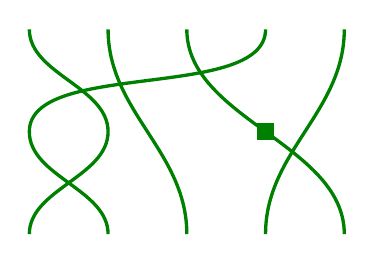
\begin{tikzpicture}[baseline,very thick,green!50!black, xscale=2,yscale=1.3]
 \draw (-.5,-1) to[out=90,in=-90] (-1,0) to[out=90,in=-90](.5,1);
 \draw (.5,-1) to[out=90,in=-90] (1,1);
 \draw (1,-1) to[out=90,in=-90] 
 node[midway,fill=green!50!black,inner sep=3pt]{} (0,1);
 \draw (-1, -1) to[out=90,in=-90] (-.5,0) to[out=90,in=-90] (-1,1);
 \draw (0,-1) to[out=90,in=-90] (-.5,1);
\end{tikzpicture}\]
As usual, we can compose these by taking $ab$ to be the diagram where
we place $a$ on top of $b$ and attempt to match up the bottom of $a$
and top of $b$. If the number of strands is the same, the result is
unique up to isotopy, and if it is different, we formally declare the
result to be $0$.



The rank $n$ \emph{type O affine Hecke algebra} is the quotient of the
span of these diagrams over $\K\llbracket h\rrbracket $ by the local relations:\newseq
%\begin{figure}[h!]
\begin{equation*}\subeqn\label{Hecke-1}
 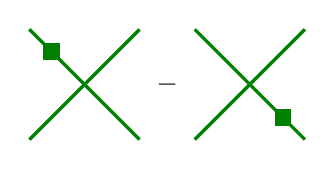
\begin{tikzpicture}[scale=.7,baseline]
 \draw[very thick,green!50!black](-3,0) +(-1,-1) -- +(1,1); \draw[very thick,green!50!black](-3,0) +(1,-1) --
 node[pos=.8,fill=green!50!black,inner sep=3pt]{} +(-1,1) ;
 % \draw[very thick] (0,0) +(0,-1) -- +(0,1) node[below, at
 % start]{$i$}; \fill (0,0) circle (5pt);
 \node at (-1.5,0){$-$}; \draw[very thick,green!50!black](0,0) +(-1,-1) -- +(1,1); \draw[very thick,green!50!black](0,0) +(1,-1) -- node[pos=.2,fill=green!50!black,inner sep=3pt]{}
 +(-1,1); 
 \end{tikzpicture}\hspace{4mm}=\hspace{4mm}
 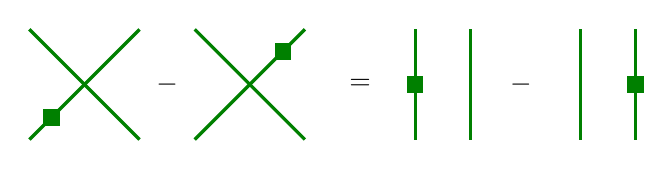
\begin{tikzpicture}[scale=.7,baseline]
 \draw[very thick,green!50!black](-3,0) +(-1,-1) -- node[pos=.2,fill=green!50!black,inner sep=3pt]{}+(1,1); \draw[very thick,green!50!black](-3,0) +(1,-1) -- +(-1,1); 
 % \draw[very thick] (0,0) +(0,-1) -- +(0,1) node[below, at
 % start]{$i$}; \fill (0,0) circle (5pt);
 \node at (-1.5,0){$-$}; \draw[very thick,green!50!black](0,0) +(-1,-1) --
 node[pos=.8,fill=green!50!black,inner sep=3pt]{} +(1,1); \draw[very thick,green!50!black](0,0) +(1,-1) -- +(-1,1)
 ; \node at (2,0){$=$}; \draw[very
 thick,green!50!black](4,0) +(-1,-1) -- node[midway,fill=green!50!black,inner
 sep=3pt]{}+(-1,1); \draw[very
 thick,green!50!black](4,0) +(0,-1) -- +(0,1); \node
 at (5,0){$-\,\,\pq$}; \draw[very thick,green!50!black](7,0) +(-1,-1) -- +(-1,1)
 ; \draw[very thick,green!50!black](7,0) +(0,-1) --
 node[midway,fill=green!50!black,inner sep=3pt]{} +(0,1);
 \end{tikzpicture}
 \end{equation*}
 \begin{equation*}\subeqn\label{Hecke-2}
 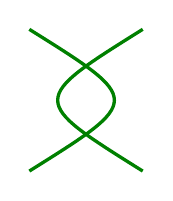
\begin{tikzpicture}[very thick,scale=.9,baseline,green!50!black]
 \draw(-2.8,0) +(0,-1) .. controls (-1.2,0) .. +(0,1)
 ; \draw (-1.2,0) +(0,-1) .. controls
 (-2.8,0) .. +(0,1) ; 
 \end{tikzpicture}\hspace{4mm}
= (1+\pq)\hspace{5mm}
 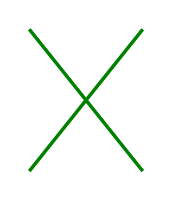
\begin{tikzpicture}[very thick,scale=.9,baseline,green!50!black]
 \draw (-2.8,-1)--(-1.2,1); \draw (-2.8,1)--(-1.2,-1); 
 \end{tikzpicture}
 \end{equation*}
 \begin{equation*}\subeqn\label{Hecke-triple}
 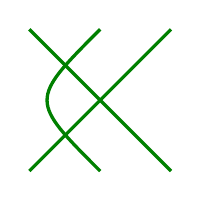
\begin{tikzpicture}[very thick,scale=.9,baseline,green!50!black]
 \draw (-3,0) +(1,-1) -- +(-1,1); \draw
 (-3,0) +(-1,-1) -- +(1,1) ; \draw
 (-3,0) +(0,-1) .. controls (-4,0) .. +(0,1); 
 \end{tikzpicture}\hspace{4mm}-\hspace{4mm}

\begin{tikzpicture}[very thick,scale=.9,baseline,green!50!black]
\draw (1,0) +(1,-1) -- +(-1,1)
 ; \draw (1,0) +(-1,-1) -- +(1,1)
 ; \draw (1,0) +(0,-1) .. controls
 (2,0) .. +(0,1); 
 \end{tikzpicture}\hspace{4mm}
= \pq \hspace{4mm} 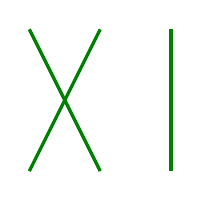
\begin{tikzpicture}[very thick,scale=.9,baseline,green!50!black]
 \draw (-3,0) +(1,-1) -- +(1,1); \draw
 (-3,0) +(-1,-1) -- +(0,1) ; \draw
 (-3,0) +(0,-1) -- +(-1,1);
 \end{tikzpicture}\hspace{4mm}-\pq \hspace{4mm} 
\begin{tikzpicture}[very thick,scale=.9,baseline,green!50!black]
 \draw (-3,0) +(-1,-1) -- +(-1,1); \draw
 (-3,0) +(1,-1) -- +(0,1) ; \draw
 (-3,0) +(0,-1) -- +(1,1);
 \end{tikzpicture}
 \end{equation*}
 \begin{rema}
 We want to make sure that the reader notices the distinction here
 between ``relations'' and ``local relations.'' Here ``relations''
 has the usual algebraic meaning: generators of the kernel of the
 homomorphism to an algebra of the free associative algebra on the
 generators. However, ``local relations'' means something a bit
 more subtle: whenever we have two diagrams which are identical
 outside a small region, and match the two sides of the equation,
 then they are set equal. Of course, the effect this has depends
 on what is allowed in the rest of the diagram.

 So a relation like
~\ref{Hecke-1} can be applied in type O diagrams (as in this
 section) or in type W diagrams, which we'll introduce later.
 While the pictures on the page are the same, the induced relations
 are different, since we have different rules for how the rest of
 the diagram is constructed. Thus in later sections, we will
 refer back to these local relations, but apply them in a different
 diagrammatic framework.
 \end{rema}
 
 \begin{rema}
 In the degenerate case, we can write a similar set of local relations,
 replacing (\ref{Hecke-1}--\ref{Hecke-triple}) with the local relations:
\begin{equation*}\subeqn\label{deg-Hecke-1}
 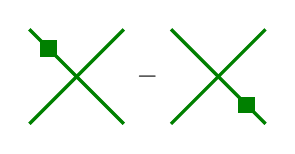
\begin{tikzpicture}[scale=.6,baseline]
 \draw[very thick,green!50!black](-3,0) +(-1,-1) -- +(1,1); \draw[very thick,green!50!black](-3,0) +(1,-1) --
 node[pos=.8,fill=green!50!black,inner sep=3pt]{} +(-1,1) ;
 % \draw[very thick] (0,0) +(0,-1) -- +(0,1) node[below, at
 % start]{$i$}; \fill (0,0) circle (5pt);
 \node at (-1.5,0){$-$}; \draw[very thick,green!50!black](0,0) +(-1,-1) -- +(1,1); \draw[very thick,green!50!black](0,0) +(1,-1) -- node[pos=.2,fill=green!50!black,inner sep=3pt]{}
 +(-1,1); 
 \end{tikzpicture}\hspace{3mm}=\hspace{3mm}
 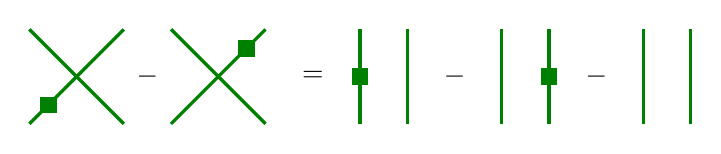
\begin{tikzpicture}[scale=.6,baseline]
 \draw[very thick,green!50!black](-3,0) +(-1,-1) -- node[pos=.2,fill=green!50!black,inner sep=3pt]{}+(1,1); \draw[very thick,green!50!black](-3,0) +(1,-1) -- +(-1,1); 
 % \draw[very thick] (0,0) +(0,-1) -- +(0,1) node[below, at
 % start]{$i$}; \fill (0,0) circle (5pt);
 \node at (-1.5,0){$-$}; \draw[very thick,green!50!black](0,0) +(-1,-1) --
 node[pos=.8,fill=green!50!black,inner sep=3pt]{} +(1,1); \draw[very thick,green!50!black](0,0) +(1,-1) -- +(-1,1)
 ; \node at (2,0){$=$}; \draw[very
 thick,green!50!black](4,0) +(-1,-1) -- node[midway,fill=green!50!black,inner
 sep=3pt]{}+(-1,1); \draw[very
 thick,green!50!black](4,0) +(0,-1) -- +(0,1); \node
 at (5,0){$-$}; \draw[very thick,green!50!black](7,0) +(-1,-1) -- +(-1,1)
 ; \draw[very thick,green!50!black](7,0) +(0,-1) --
 node[midway,fill=green!50!black,inner sep=3pt]{} +(0,1); \node
 at (8,0){$-$};
\draw[very thick,green!50!black](10,0) +(-1,-1) -- +(-1,1)
 ; \draw[very thick,green!50!black](10,0) +(0,-1) --+(0,1);
 \end{tikzpicture}
 \end{equation*}
 \begin{equation*}\subeqn\label{deg-Hecke-2}
 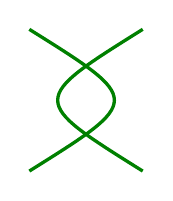
\begin{tikzpicture}[very thick,scale=.9,baseline,green!50!black]
 \draw(-2.8,0) +(0,-1) .. controls (-1.2,0) .. +(0,1)
 ; \draw (-1.2,0) +(0,-1) .. controls
 (-2.8,0) .. +(0,1) ; 
 \end{tikzpicture}\hspace{4mm}
= \,\,2\hspace{5mm}
 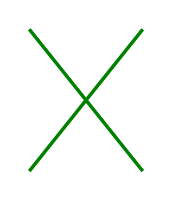
\begin{tikzpicture}[very thick,scale=.9,baseline,green!50!black]
 \draw (-2.8,-1)--(-1.2,1); \draw (-2.8,1)--(-1.2,-1); 
 \end{tikzpicture}
 \end{equation*}
 \begin{equation*}\subeqn\label{deg-Hecke-triple}
 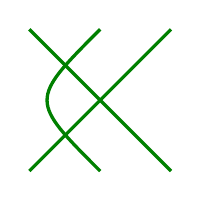
\begin{tikzpicture}[very thick,scale=.9,baseline,green!50!black]
 \draw (-3,0) +(1,-1) -- +(-1,1); \draw
 (-3,0) +(-1,-1) -- +(1,1) ; \draw
 (-3,0) +(0,-1) .. controls (-4,0) .. +(0,1); 
 \end{tikzpicture}\hspace{4mm}-\hspace{4mm}

\begin{tikzpicture}[very thick,scale=.9,baseline,green!50!black]
\draw (1,0) +(1,-1) -- +(-1,1)
 ; \draw (1,0) +(-1,-1) -- +(1,1)
 ; \draw (1,0) +(0,-1) .. controls
 (2,0) .. +(0,1); 
 \end{tikzpicture}\hspace{4mm}
= \hspace{4mm} 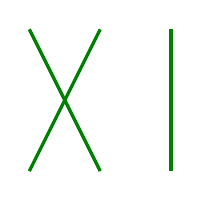
\begin{tikzpicture}[very thick,scale=.9,baseline,green!50!black]
 \draw (-3,0) +(1,-1) -- +(1,1); \draw
 (-3,0) +(-1,-1) -- +(0,1) ; \draw
 (-3,0) +(0,-1) -- +(-1,1);
 \end{tikzpicture}\hspace{4mm}- \hspace{4mm} 
\begin{tikzpicture}[very thick,scale=.9,baseline,green!50!black]
 \draw (-3,0) +(-1,-1) -- +(-1,1); \draw
 (-3,0) +(1,-1) -- +(0,1) ; \draw
 (-3,0) +(0,-1) -- +(1,1);
 \end{tikzpicture}
 \end{equation*}
 \end{rema}

It may not be immediately clear what the additional value of this graphical
presentations is. However, this perspective
will lead us to generalizations of the affine Hecke algebra which we
call types W, F and WF.
 \begin{theorem}\label{type-O-Hecke}
The algebra $\gls{mH}(\pq)$ is isomorphic to the rank $n$ type O Hecke
algebra via the map sending $T_r+1$ to the crossing of the $r$th and
$r+1$st strands, and $X_r$ to the square on the $r$th strand, as shown below:
%The map sending $-T_{n-r-1}+q$ to the same crossing and
%$q^{2r-2}X_{n-r}$ to the the square on the $r$th strand is an
%anti-isomorphism.
 \begin{equation}\label{Hecke-gens}
 \tikz[baseline]{
 \node[label=below:{$X_j$}] at (0,0){ 
 \tikz[very thick,xscale=1.2,green!50!black]{
 \draw (-.5,-.5)-- (-.5,.5);
 \draw (.5,-.5)-- (.5,.5) node [midway,fill=green!50!black,inner
 sep=2.5pt]{};
 \draw (1.5,-.5)-- (1.5,.5);
 \node at (1,0){$\cdots$};
 \node at (0,0){$\cdots$};
 }
 };
 \node[label=below:{$T_j+1$}] at (4.5,0){ 
 \tikz[very thick,xscale=1.2, green!50!black]{
 \draw (-.5,-.5)-- (-.5,.5);
 \draw (.1,-.5)-- (.9,.5);
 \draw (.9,-.5)-- (.1,.5);
 \draw (1.5,-.5)-- (1.5,.5);
 \node at (1,0){$\cdots$};
 \node at (0,0){$\cdots$};
 }
 };
 }\vspace{-2mm}
 \end{equation}
 \end{theorem}
%We'll call these two isomorphisms the $+$-isomorphism and the $-$-isomorphism.
 \begin{proof}
\newseq
 We'll use the relations given in~\cite[\S~4]{BKKL} without
 additional citation. The
 equations (\ref{Hecke-1}--\ref{Hecke-triple}) become the relations: 
\begin{gather*}
 \begin{aligned}
 X_r(T_r+1)-(T_r+1)X_{r+1}
 &=T_rX_{r+1}+(1-\pq)X_{r+1}+X_r-T_rX_{r+1}-X_{r+1} \\ 
 &=X_r-\pq X_{r+1}\\
 X_{r+1}(T_r+1)-(T_r+1)X_{r}
 &=T_rX_{r}+(\pq-1)X_{r+1}+X_{r+1}-T_rX_{r}-X_{r}\\
 &=qX_{r+1}-X_r\\
 (T_r+1)^2&=T_r^2+2T_r+1\\
&=(\pq-1)T_r+\pq+2T_r+1\\
&=(1+\pq)(T_r+1)
 \end{aligned}
 \\
 \begin{aligned}
 (T_r+1)(T_{r+1}+1)(T_r+1)-(T_{r+1}+1)(T_{r}+1)(T_{r+1}+1)&=
 T_r^2+T_r-T_{r+1}^2 -T_{r+1}\\
 &=\pq(T_r-T_{r+1}).
 \end{aligned}
 \end{gather*}
Similarly, one can easily derive the relations of the affine Hecke
from the diagrammatic ones given above. This shows that we have an
isomorphism.
 \end{proof}
Note that if we instead sent the element $T_i-\pq$ to the crossing, we
would obtain local relations which are quite similar to
(\ref{Hecke-1}--\ref{Hecke-triple}), but have a few subtle
differences:
\begin{equation*}\subeqn\label{qHecke-1}
 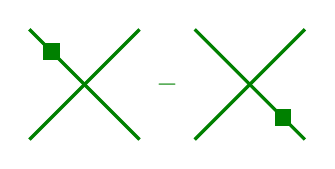
\begin{tikzpicture}[scale=.7,baseline,green!50!black]
 \draw[very thick](-3,0) +(-1,-1) -- +(1,1); \draw[very thick](-3,0) +(1,-1) --
 node[pos=.8,fill=green!50!black,inner sep=3pt]{} +(-1,1) ;
 % \draw[very thick] (0,0) +(0,-1) -- +(0,1) node[below, at
 % start]{$i$}; \fill (0,0) circle (5pt);
 \node at (-1.5,0){$-$}; \draw[very thick](0,0) +(-1,-1) -- +(1,1); \draw[very thick](0,0) +(1,-1) -- node[pos=.2,fill=green!50!black,inner sep=3pt]{}
 +(-1,1); 
 \end{tikzpicture}\hspace{4mm}=\hspace{4mm}
 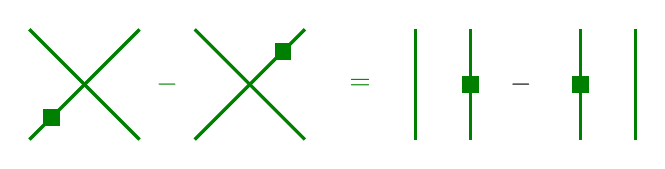
\begin{tikzpicture}[scale=.7,baseline,green!50!black]
 \draw[very thick](-3,0) +(-1,-1) -- node[pos=.2,fill=green!50!black,inner sep=3pt]{}+(1,1); \draw[very thick](-3,0) +(1,-1) -- +(-1,1); 
 % \draw[very thick] (0,0) +(0,-1) -- +(0,1) node[below, at
 % start]{$i$}; \fill (0,0) circle (5pt);
 \node at (-1.5,0){$-$}; \draw[very thick](0,0) +(-1,-1) --
 node[pos=.8,fill=green!50!black,inner sep=3pt]{} +(1,1); \draw[very thick](0,0) +(1,-1) -- +(-1,1)
 ; \node at (2,0){$=$}; \draw[very
 thick](4,0) +(-1,-1) -- +(-1,1); \draw[very
 thick](4,0) +(0,-1) -- node[midway,fill=green!50!black,inner
 sep=3pt]{}+(0,1); \node[black]
 at (5,0){$-\,\,\pq$}; \draw[very thick](7,0) +(-1,-1) -- node[midway,fill=green!50!black,inner sep=3pt]{}+(-1,1)
 ; \draw[very thick](7,0) +(0,-1) --
 +(0,1);
 \end{tikzpicture}
 \end{equation*}
 \begin{equation*}\subeqn\label{qHecke-2}
 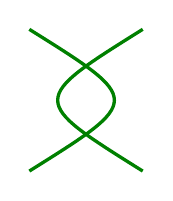
\begin{tikzpicture}[very thick,scale=.9,baseline,green!50!black]
 \draw(-2.8,0) +(0,-1) .. controls (-1.2,0) .. +(0,1)
 ; \draw (-1.2,0) +(0,-1) .. controls
 (-2.8,0) .. +(0,1) ; 
 \end{tikzpicture}\hspace{4mm}
= -(1+\pq)\hspace{5mm}
 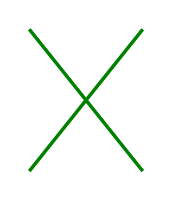
\begin{tikzpicture}[very thick,scale=.9,baseline,green!50!black]
 \draw (-2.8,-1)--(-1.2,1); \draw (-2.8,1)--(-1.2,-1); 
 \end{tikzpicture}
 \end{equation*}
 \begin{equation*}\subeqn\label{qHecke-triple}
 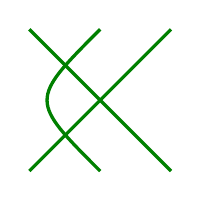
\begin{tikzpicture}[very thick,scale=.9,baseline,green!50!black]
 \draw (-3,0) +(1,-1) -- +(-1,1); \draw
 (-3,0) +(-1,-1) -- +(1,1) ; \draw
 (-3,0) +(0,-1) .. controls (-4,0) .. +(0,1); 
 \end{tikzpicture}\hspace{4mm}-\hspace{4mm}

\begin{tikzpicture}[very thick,scale=.9,baseline,green!50!black]
\draw (1,0) +(1,-1) -- +(-1,1)
 ; \draw (1,0) +(-1,-1) -- +(1,1)
 ; \draw (1,0) +(0,-1) .. controls
 (2,0) .. +(0,1); 
 \end{tikzpicture}\hspace{4mm}
= \pq \hspace{4mm} 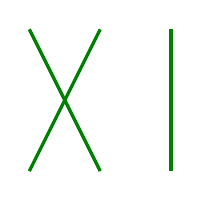
\begin{tikzpicture}[very thick,scale=.9,baseline,green!50!black]
 \draw (-3,0) +(1,-1) -- +(1,1); \draw
 (-3,0) +(-1,-1) -- +(0,1) ; \draw
 (-3,0) +(0,-1) -- +(-1,1);
 \end{tikzpicture}\hspace{4mm}-\pq \hspace{4mm} 
\begin{tikzpicture}[very thick,scale=.9,baseline,green!50!black]
 \draw (-3,0) +(-1,-1) -- +(-1,1); \draw
 (-3,0) +(1,-1) -- +(0,1) ; \draw
 (-3,0) +(0,-1) -- +(1,1);
 \end{tikzpicture}
 \end{equation*}
Our first task is to describe the completions that are of interest to
us.



Consider a finite subset
$\gls{U}\subset \K\setminus\{0\}$; as before, we endow this with a graph structure by adding an edge
from $u$ to $u'$ if $u'=qu$. Note that for $\gls{U}$
chosen generically there will simply be no edges, and that under this
graph structure $\gls{U}$ will always be a union of segments and cycles with $e$
nodes (if $e<\infty$).

We will apply the results of Section~\ref{sec:polyn-style-repr} in
this context with
\begin{equation}
\mathbb{K}=\K\llbracket h\rrbracket \qquad A=\mH(\pq)\qquad
 B=\K\llbracket h\rrbracket [X^{\pm}]\qquad I=Bh+B \prod_{u\in \gls{U}}(X-u).\label{eq:Hecke-PR}
\end{equation}


One natural construction of modules over $\gls{mH}(\pq)$ is given by
induction from $\gls{mHfin} $, as discussed in~\cite[\S~4.3]{MacHecke}; as discussed there, the result is free as a
$\mathcal{C}$-module if the original module is free over $\K\llbracket h\rrbracket $,
with ranks matching. In particular, applying this to the two 1-dimensional
representations of $\gls{mHfin}$, where this algebra acts by the
characters $\chi^\pm$ where
\[ \chi^+(T_i)=\pq\qquad \chi^-(T_i)=-1\] gives natural (signed) polynomial
representation \[\cP^\pm=\gls{mH}(\pq)\otimes_{\gls{mHfin}}\K\llbracket h\rrbracket ;\] where
$\gls{mHfin}$ acts on $\K\llbracket h\rrbracket $ via the homomorphism $\chi^\pm$.
\begin{lemma}
 The data of~\eqref{eq:Hecke-PR} defines a polynomial-style
 representation on $P=\cP^{\pm}$. 
\end{lemma}
\begin{proof}\mbox{}
 \begin{enumerate}
 \item This freeness is clear from the basis in
~\cite[4.3]{MacBourbaki}; in fact, as
 $B^{\otimes n}=\mathcal{C}$-module, we have
 $\gls{mH}(\pq)\cong \mathcal{C}\otimes_{\K\llbracket h\rrbracket }\gls{mHfin} $. 
 \item The center of the affine Hecke algebra $\gls{mH}(\pq)$ is precisely
 the symmetric Laurent polynomials $Z=\mathcal{C}^{S_n}$ by
~\cite[4.5]{MacBourbaki}.
 \item The module $\cP^{\pm}$ is faithful by
~\cite[(4.3.10)]{MacHecke}, and its freeness over $\mathcal{C}$
 has already been discussed.\qedhere
 \end{enumerate}
\end{proof}


Thus, as in Section~\ref{sec:polyn-style-repr}, we have an induced
topology on $\mH(\pq)$ with completion $\hmH(\pq)$. We could also
define $\hmH(\pq)$ as the completion of
$\gls{mH}(\pq)$ in the directed system of all quotients where the spectrum of
each $X_i$ lies in $\gls{U}$. 

We can
identify $\Spec(\mathcal{C})$ with $(\mathbb{A}^1\setminus
\{0\})^n\times \widehat{\mathbb{A}}^1$ where the last factor has coordinate
$h$ and is completed at $0$. 
 Let $\mathcal{U}=\gls{U}^n\times \{0\}\subset \Spec(\mathcal{C})$. This
 is the vanishing set of $I^{(n)}$ as defined in Section
~\ref{sec:polyn-style-repr}. Thus, the closure of $\mathcal{C}$ in
 $\hmH(\pq)$ is the completion of $\mathcal{C}$ at this subscheme. In
 particular, the identity in $\mathcal{C}$, and thus in $\hmH(\pq)$
 decomposes as a sum of idempotents $1=\sum_{\Bu\in \gls{U}^n}e_{\Bu}$. These have the
 property that on any topological $\hmH(\pq)$-module $M$, we have that 
\[e_{\Bu}M=\{ g\in M \mid\lim_{N\to \infty}
 (X_j-{u_j})^Ng=0\},\]
and for any module, we have $M=\oplus e_{\Bu}M$. 

%In the quotient $\hmH_0$, we have that $X_i$ acts on the quotient
%$\gls{mH}_0/\cJ_n$ with minimal polynomial dividing $\prod_{u\in
% U}(X_i-u)^n$ and thus 
%spectrum $U$. In fact, 
%Each quotient $\gls{mH}_0/\cJ_n$ is the sum of the simultaneous stable kernels
%of the elements $X_i-u_i$ for $(u_1,\dots, u_n)\in U^n$.

In particular,
we have that $\hmH(\pq)=\bigoplus_{\Bu\in \gls{U}^n}e_{\Bu}\hmH(\pq)=\bigoplus_{\Bu,\Bu'\in \gls{U}^n}e_{\Bu}\hmH(\pq) e_{\Bu'}$. 

\subsubsection{Formulas for the polynomial representation}
\label{sec:form-polyn-repr}


Now, let us study the action of $\mH(\pq)$ on its polynomial
representation $\cP^{\pm}$. Denote the action of $S_n$ on $\gls{U}^n$ by $\Bu\mapsto \Bu^s$ for $s\in
S_n$; as usual, we let $s_i=(i, i+1)$. For any Laurent polynomial $F$,
we let $F^{s_r}(X_1,\dots,X_n)=F(X_1,\dots,X_{r+1},X_r,\dots, X_n)$. 

For notational clarity, we denote $\hone=1\otimes 1\in \cP^-$, so this
representation is generated by this vector, subject to the relation
$T_i \hone=-\hone$. As in~\cite[(4.3.3)]{MacHecke}, one can calculate the action of $T_i$ on
$F \hone$ 
for any Laurent polynomial $F$; this is easiest to see if we expand
$F=F_0+(X_i-X_{i+1})F_1$ where $F_0$ and $F_1$ are $s_i$-invariant
Laurent polynomials. Thus, we have that 
\begin{align*}
 T_i F\hone&= T_i F_0\hone+T_i(X_i-X_{i+1})F_1\hone\\
 &=-F_0\hone+(X_i-X_{i+1})F_1\hone+2(1-\pq)
X_{i+1}F_1\hone\\
&= -F^{s_i}\hone+ (1-\pq)
X_{i+1}\frac{F^{s_i}-F}{X_{i+1}-X_i}\hone.
\end{align*}
Thus, we have that 
\[(T_i+1) F\hone =\left(F-F^{s_i}+ (1-\pq)
X_{i+1}\frac{F^{s_i}-F}{X_{i+1}-X_i}\right)\hone+\frac{X_i-\pq X_{i+1}}{X_{i+1}-X_i} (F^{s_i}-F)\hone.\]

The Hecke algebra acts faithfully on this
representation by~\cite[(4.3.10)]{MacHecke}, so we can identify the affine Hecke algebra with a
subalgebra of operators on $\cP^\pm$.

Similarly, the representation $\cP^+$ is
generated by an element $\hone^+$ satisfying $T_i\hone^+=\pq \hone^+$.
The action of $\gls{mH}(\pq)$ in this case is given by the formula
\[T_iF\hone^+=\pq F^{s_i}\hone^++(1-\pq)X_{i+1}\frac{F^{s_i}-F}{X_{i+1}-X_i}\hone^+\]
so we have that 
\[(T_i-\pq)\hone^+=\frac{X_{i+1}-\pq X_i}{X_{i+1}-X_i}( F^{s_i}-F).\]

Consider the $\hmH(\pq)$-module $\hcP^\pm :=\hmH(\pq)
\otimes_{\gls{mH}(\pq)}\cP^\pm$. It follows from Lemma
\ref{lem:faithful-completion} that:
\begin{lemma}\label{lem:Hecke-P}
 The module $\hcP^\pm$ is a rank 1 free module over the completion
 of $\mathcal{C} $ at the set $\mathcal{U}$, and this
 representation remains faithful. The space $e_{\Bu}\hcP^\pm $ is isomorphic to
$\K\llbracket (X_1-{u_1}),\dots, (X_n-{u_n}),h\rrbracket $ via the action map on
$e_{\Bu}\hone$.
 \end{lemma}

\subsection{KLR algebras}

We wish to define a similar completion of the KLR algebra $\gls{R}(h)$ for the
graph $\gls{U}$. We use the conventions of Brundan and Kleshchev, but we
record the relations we need here for the sake of completeness and to
match our slightly more general context. The rank\footnote{Note here
 that the ``rank'' $n$ has no relationship to the size of the set $\gls{U}$
(typically called the rank of the corresponding Kac--Moody algebra);
for any fixed $\gls{U}$, we get a different algebra for each positive
integer $n$.} $n$ KLR algebra $\gls{R}(h)$ attached to the Dynkin
diagram $\gls{U}$ is
generated over $\K[h]$ 
by elements $\{e(\Bu)\}_{\Bu\in \gls{U}^n}\cup \{y_1,\dots, y_n\}\cup \{\psi_1,\dots, \psi_{n-1}\}$
subject to the relations:
\begin{align*}
e(\Bu) e(\Bv) &= \delta_{\Bu,\Bv} e(\Bu);
\hspace{53mm}{\sum_{\Bu \in I^\alpha}} e(\Bu) = 1;\\
y_r e(\Bu) &= e(\Bu) y_r;
\hspace{53mm}\psi_r e(\Bu) = e(\Bu^{s_r}) \psi_r;\\
y_r y_s &= y_s y_r;\\
\psi_r y_s &= y_s \psi_r\hspace{61.4mm}\text{if $s \neq r,r+1$};\\
\psi_r \psi_s &= \psi_s \psi_r\hspace{60.8mm}\text{if $s\neq r\pm 1$};\\
\psi_r y_{r+1} e(\Bu) 
&= 
\begin{cases}
 (y_r\psi_r+1)e(\Bu) &\hbox{if $u_r=u_{r+1}$},\\
 y_r\psi_r e(\Bu) \hspace{48mm}&\hbox{if $u_r\neq u_{r+1}$};
\end{cases}\\
y_{r+1} \psi_re(\Bu) &=
\begin{cases}
 (\psi_r y_r+1) e(\Bu)
 &\hbox{if $u_r=u_{r+1}$},\\
 \psi_r y_r e(\Bu) \hspace{48mm}&\hbox{if $u_r\neq u_{r+1}$};\\
\end{cases}\\
\psi_r^2e(\Bu) &=
\begin{cases}
0 \hspace{60mm}&\text{if $u_r = u_{r+1}$},\\
e(\Bu)&\text{if $u_r \neq q^{\pm 1}u_{r+1},u_{r+1}$},\\
(y_{r+1}-y_r+d_1h)e(\Bu)&\text{if $u_r = q^{-1}u_{r+1}, q\neq -1$},\\
(y_r - y_{r+1}+d_1h)e(\Bu)&\text{if $u_r = qu_{r+1}, q\neq -1$},\\
(y_r - y_{r+1}+d_1h)(y_{r+1} - y_{r}+d_1h) e(\Bu)&\text{if $u_r=-u_{r+1}, q=-1$};
\end{cases}
\end{align*}\begin{multline*}
\psi_{r}\psi_{r + 1} \psi_{r} e(\Bu)
\\
=
\begin{cases}
 (\psi_{r\Mk+ 1} \psi_{r} \psi_{r + 1}  + 1)e(\Bu)& \text{if $u_r  =  u_{r + 2} = q^{-1}u_{r + 1}, q \neq  -1$},\\
 (\psi_{r+1} \psi_{r} \psi_{r+1} -1)e(\Bu)& \text{if $u_r = u_{r+2}=qu_{r+1}, q\neq -1$},\\
 \big(\psi_{r+1} \psi_{r} \psi_{r+1} -2y_{r+1} +y_r+y_{r+2}\big)e(\Bu)
& \text{if $u_r = u_{r+2}=-u_{r+1}, q= -1$},\\
 \psi_{r+1} \psi_{r} \psi_{r+1} e(\Bu)& \text{otherwise}.
\end{cases}
\end{multline*}

Just as in the Hecke case, there is a graphical
presentation for the KLR algebra. Since this is covered in~\cite{KLI}
and numerous other sources, we'll just record an example of an
appropriate KLR diagram here for comparison purposes:\newseq 
\[
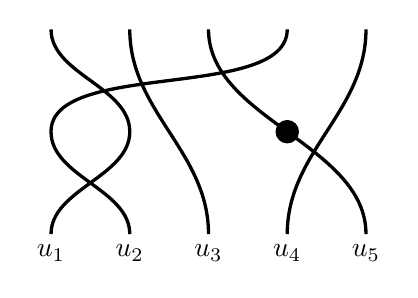
\begin{tikzpicture}[baseline,very thick,xscale=2,yscale=1.3]
 \draw (-.5,-1) to[out=90,in=-90] node[below,at start]{$u_2$} (-1,0) to[out=90,in=-90](.5,1);
 \draw (.5,-1) to[out=90,in=-90] node[below,at start]{$u_4$} (1,1);
 \draw (1,-1) to[out=90,in=-90] node[below,at start]{$u_5$}
 node[circle, midway,fill=black,inner sep=3pt]{} (0,1);
 \draw (-1, -1) to[out=90,in=-90]node[below,at start]{$u_1$} (-.5,0) to[out=90,in=-90] (-1,1);
 \draw (0,-1) to[out=90,in=-90] node[below,at start]{$u_3$} (-.5,1);
\end{tikzpicture}\] 
and write out the local relations here for convenience:
\begin{equation*}
\subeqn\label{first-QH} %%%%% 5a
 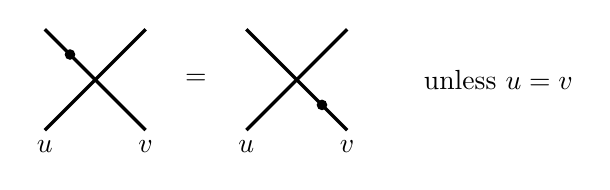
\begin{tikzpicture}[scale=.64,baseline]
 \draw[very thick](-4,0) +(-1,-1) -- +(1,1) node[below,at start]
 {$u$}; \draw[very thick](-4,0) +(1,-1) -- +(-1,1) node[below,at
 start] {$v$}; \fill (-4.5,.5) circle (3pt);
 % \draw[very thick] (0,0) +(0,-1) -- +(0,1) node[below, at
 % start]{$u$}; \fill (0,0) circle (5pt);
 \node at (-2,0){=}; \draw[very thick](0,0) +(-1,-1) -- +(1,1)
 node[below,at start] {$u$}; \draw[very thick](0,0) +(1,-1) --
 +(-1,1) node[below,at start] {$v$}; \fill (.5,-.5) circle (3pt);
 \node at (4,0){unless $u=v$};
 \end{tikzpicture}
 \end{equation*}
\begin{equation*}\subeqn  %%%%% 5b
 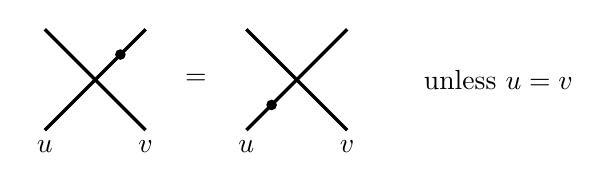
\begin{tikzpicture}[scale=.64,baseline]
 \draw[very thick](-4,0) +(-1,-1) -- +(1,1) node[below,at start]
 {$u$}; \draw[very thick](-4,0) +(1,-1) -- +(-1,1) node[below,at
 start] {$v$}; \fill (-3.5,.5) circle (3pt);
 % \draw[very thick] (0,0) +(0,-1) -- +(0,1) node[below, at
 % start]{$u$}; \fill (0,0) circle (5pt);
 \node at (-2,0){=}; \draw[very thick](0,0) +(-1,-1) -- +(1,1)
 node[below,at start] {$u$}; \draw[very thick](0,0) +(1,-1) --
 +(-1,1) node[below,at start] {$v$}; \fill (-.5,-.5) circle (3pt);
 \node at (4,0){unless $u=v$};
 \end{tikzpicture}
 \end{equation*}
\begin{equation*}\subeqn\label{nilHecke-1}  %%%%% 5c
 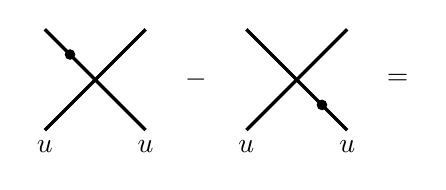
\begin{tikzpicture}[scale=.64,baseline]
 \draw[very thick](-4,0) +(-1,-1) -- +(1,1) node[below,at start]
 {$u$}; \draw[very thick](-4,0) +(1,-1) -- +(-1,1) node[below,at
 start] {$u$}; \fill (-4.5,.5) circle (3pt);
 % \draw[very thick] (0,0) +(0,-1) -- +(0,1) node[below, at
 % start]{$u$}; \fill (0,0) circle (5pt);
 \node at (-2,-0){$-$}; \draw[very thick](0,0) +(-1,-1) -- +(1,1)
 node[below,at start] {$u$}; \draw[very thick](0,0) +(1,-1) --
 +(-1,1) node[below,at start] {$u$}; \fill (.5,-.5) circle (3pt);
 \node at (2,0){$=$}; 
 \end{tikzpicture}
 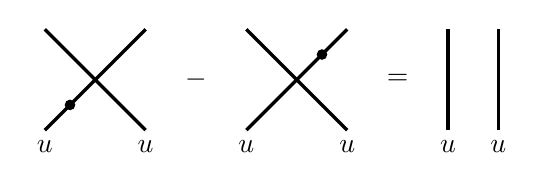
\begin{tikzpicture}[scale=.64,baseline]
 \draw[very thick](-4,0) +(-1,-1) -- +(1,1) node[below,at start]
 {$u$}; \draw[very thick](-4,0) +(1,-1) -- +(-1,1) node[below,at
 start] {$u$}; \fill (-4.5,-.5) circle (3pt);
 % \draw[very thick] (0,0) +(0,-1) -- +(0,1) node[below, at
 % start]{$u$}; \fill (0,0) circle (5pt);
 \node at (-2,0){$-$}; \draw[very thick](0,0) +(-1,-1) -- +(1,1)
 node[below,at start] {$u$}; \draw[very thick](0,0) +(1,-1) --
 +(-1,1) node[below,at start] {$u$}; \fill (.5,.5) circle (3pt);
 \node at (2,0){$=$}; \draw[very thick](4,0) +(-1,-1) -- +(-1,1)
 node[below,at start] {$u$}; \draw[very thick](4,0) +(0,-1) --
 +(0,1) node[below,at start] {$u$};
 \end{tikzpicture}
 \end{equation*}
\refstepcounter{subeqn}
\begin{multline*}\subeqn\label{black-bigon}
 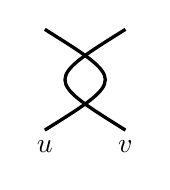
\begin{tikzpicture}[very thick,scale=.64,baseline]
 \draw (-2.8,0) +(0,-1) .. controls (-1.2,0) .. +(0,1)
 node[below,at start]{$u$}; \draw (-1.2,0) +(0,-1) .. controls
 (-2.8,0) .. +(0,1) node[below,at start]{$v$}; 
 \end{tikzpicture}\\
 =
 \begin{cases}
0 & u\Mk =\Mk v\\
 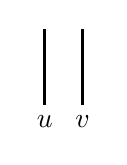
\begin{tikzpicture}[very thick,scale=.48,baseline=-3pt]
 \draw (2,0) +(0,-1) -- +(0,1) node[below,at start]{$v$};
 \draw (1,0) +(0,-1) -- +(0,1) node[below,at start]{$u$};
 \end{tikzpicture} & u\Mk \notin \Mk \{v,qv,q^{-1}v\}\\
 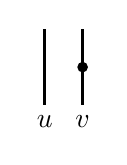
\begin{tikzpicture}[very thick,scale=.48,baseline=-3pt]
 \draw (2,0) +(0,-1) -- +(0,1) node[below,at start]{$v$};
 \draw (1,0) +(0,-1) -- +(0,1) node[below,at start]{$u$};\fill (2,0) circle (4pt);
 \end{tikzpicture}-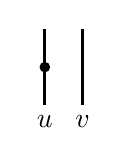
\begin{tikzpicture}[very thick,scale=.48,baseline=-3pt]
 \draw (2,0) +(0,-1) -- +(0,1) node[below,at start]{$v$};
 \draw (1,0) +(0,-1) -- +(0,1) node[below,at start]{$u$};\fill (1,0) circle (4pt);
 \end{tikzpicture}+d_1h 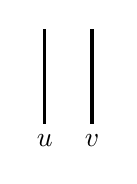
\begin{tikzpicture}[very thick,scale=.6,baseline=-3pt]
 \draw (2,0) +(0,-1) -- +(0,1) node[below,at start]{$v$};
 \draw (1,0) +(0,-1) -- +(0,1) node[below,at start]{$u$};
 \end{tikzpicture}& u\Mk =\Mk q^{-1}v,q\Mk \neq \Mk -\Mk 1\\
 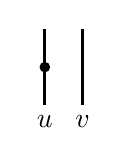
\begin{tikzpicture}[very thick,baseline=-3pt,scale=.48]
 \draw (2,0) +(0,-1) -- +(0,1) node[below,at start]{$v$};
 \draw (1,0) +(0,-1) -- +(0,1) node[below,at start]{$u$};\fill (1,0) circle (4pt);
 \end{tikzpicture}-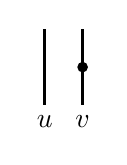
\begin{tikzpicture}[very thick,scale=.48,baseline=-3pt]
 \draw (2,0) +(0,-1) -- +(0,1) node[below,at start]{$v$};
 \draw (1,0) +(0,-1) -- +(0,1) node[below,at start]{$u$};\fill (2,0) circle (4pt);
 \end{tikzpicture}+d_1h 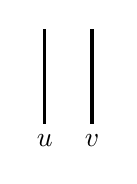
\begin{tikzpicture}[very thick,scale=.6,baseline=-3pt]
 \draw (2,0) +(0,-1) -- +(0,1) node[below,at start]{$v$};
 \draw (1,0) +(0,-1) -- +(0,1) node[below,at start]{$u$};
 \end{tikzpicture}& u\Mk =\Mk qv,q\Mk \neq \Mk -\Mk 1\\
 - \Bigg(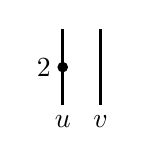
\begin{tikzpicture}[very thick,scale=.48,baseline=-3pt]
 \draw (2,0) +(0,-1) -- +(0,1) node[below,at start]{$v$};
 \draw (1,0) +(0,-1) -- +(0,1) node[below,at start]{$u$};\fill
 (1,0) circle (4pt); \node at (.5,0) {$2$};
 \end{tikzpicture}\Bigg)+2 \Bigg(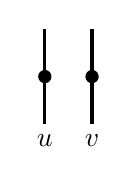
\begin{tikzpicture}[very thick,scale=.6,baseline=-3pt]
 \draw (2,0) +(0,-1) -- +(0,1) node[below,at start]{$v$};
 \draw (1,0) +(0,-1) -- +(0,1) node[below,at start]{$u$};\fill (2,0) circle (4pt);\fill (1,0) circle (4pt);
 \end{tikzpicture}\Bigg)- \Bigg(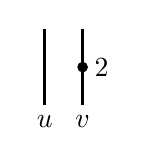
\begin{tikzpicture}[very thick,scale=.48,baseline=-3pt]
 \draw (2,0) +(0,-1) -- +(0,1) node[below,at start]{$v$};
 \draw (1,0) +(0,-1) -- +(0,1) node[below,at start]{$u$};\fill
 (2,0) circle (4pt); \node at (2.5,0) {$2$}; \end{tikzpicture}\Bigg)+d_1^2h^2 \Bigg(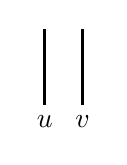
\begin{tikzpicture}[very thick,scale=.48,baseline=-3pt]
 \draw (2,0) +(0,-1) -- +(0,1) node[below,at start]{$v$};
 \draw (1,0) +(0,-1) -- +(0,1) node[below,at start]{$u$};
 \end{tikzpicture}\Bigg)& u\Mk =\Mk -v,q\Mk =\Mk -1
 \end{cases}
 \end{multline*}
\addtocounter{subeqn}{-1}
 \begin{equation*}\subeqn\label{triple-dumb}
 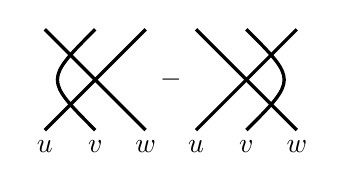
\begin{tikzpicture}[very thick,scale=.64,baseline=-3pt]
 \draw (-2,0) +(1,-1) -- +(-1,1) node[below,at start]{$w$}; \draw
 (-2,0) +(-1,-1) -- +(1,1) node[below,at start]{$u$}; \draw
 (-2,0) +(0,-1) .. controls (-3,0) .. +(0,1) node[below,at
 start]{$v$}; \node at (-.5,0) {$-$}; \draw (1,0) +(1,-1) -- +(-1,1)
 node[below,at start]{$w$}; \draw (1,0) +(-1,-1) -- +(1,1)
 node[below,at start]{$u$}; \draw (1,0) +(0,-1) .. controls
 (2,0) .. +(0,1) node[below,at start]{$v$}; \end{tikzpicture}=\quad
 \begin{cases} 
 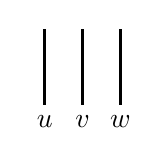
\begin{tikzpicture}[very thick,scale=.48,baseline=-3pt]
 \draw (6.2,0)
 +(1,-1) -- +(1,1) node[below,at start]{$w$}; \draw (6.2,0)
 +(-1,-1) -- +(-1,1) node[below,at start]{$u$}; \draw (6.2,0)
 +(0,-1) -- +(0,1) node[below,at
 start]{$v$}; \end{tikzpicture}& u=w=qv,q\neq -1\\
 -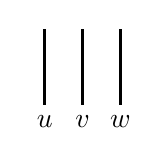
\begin{tikzpicture}[very thick,scale=.48,baseline]
 \draw (6.2,0)
 +(1,-1) -- +(1,1) node[below,at start]{$w$}; \draw (6.2,0)
 +(-1,-1) -- +(-1,1) node[below,at start]{$u$}; \draw (6.2,0)
 +(0,-1) -- +(0,1) node[below,at
 start]{$v$}; \end{tikzpicture}& u=w=q^{-1}v,q\neq -1\\
 -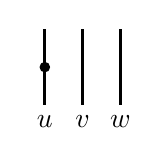
\begin{tikzpicture}[very thick,scale=.48,baseline=-3pt]
 \draw (0,0)
 +(1,-1) -- +(1,1) node[below,at start]{$w$}; \draw (0,0)
 +(-1,-1) -- +(-1,1) node[below,at start]{$u$}; \draw (0,0)
 +(0,-1) -- +(0,1) node[below,at
 start]{$v$}; \fill
 (-1,0) circle (4pt); \end{tikzpicture}-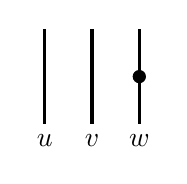
\begin{tikzpicture}[very thick,scale=.6,baseline]
 \draw (0,0)
 +(1,-1) -- +(1,1) node[below,at start]{$w$}; \draw (0,0)
 +(-1,-1) -- +(-1,1) node[below,at start]{$u$}; \draw (0,0)
 +(0,-1) -- +(0,1) node[below,at
 start]{$v$}; \fill
 (1,0) circle (4pt); \end{tikzpicture}& u=w=-v,q= -1.
 \end{cases}
 \end{equation*}

 
We will again apply the results of Section~\ref{sec:polyn-style-repr},
now with 
\begin{equation}
\mathbb{K}=\K[h]\qquad A=\gls{R}(h)\qquad
 B=\K[h,y]\qquad I=Bh+By.\label{eq:KLR-PR}
\end{equation}
We let $C=B^{\otimes n}=\K[y_1,\dots,y_n,h]=\subset \gls{R}(h)$.
The algebra $\gls{R}(h)$ also has a natural polynomial representation $P$, defined
by Rouquier
in~\cite[\S~3.2]{Rou2KM} and Khovanov and Lauda in~\cite[\S~2.3]{KLI}.
 This representation $P$ is generated
by a single element $\bone$, with the relations
\[ \psi_ke_{\Bu}\bone=
\begin{cases}
 0 & u_k=u_{k+1}\\
 (y_{k+1}-y_k+d_1h)e_{\Bu^{s_k}}\bone & u_k=qu_{k+1}\\
 e_{\Bu^{s_k}}\bone & u_k\neq u_{k+1},qu_{k+1}.
\end{cases}
\]
This can be written as a sum of the images of $e_{\Bu}$, and we always
have that $e_{\Bu}P$ is a rank 1 free module over
$C$. 

Just as in the Hecke algebra, the action of $\psi_k$ on arbitrary
polynomials can be written in terms of Demazure operators. For a
polynomial $f\in \K\llbracket h\rrbracket [y_1,\dots, y_n]$, we can describe the action
as 
\begin{equation}
 \psi_k f e_{\Bu}\bone=
\begin{cases}
 \displaystyle \frac{f^{s_k}-f}{y_{k+1}-y_k} e_{\Bu}\bone& u_k=u_{k+1}\\
 (y_{k+1}-y_k+d_1h)f^{s_k}e_{\Bu^{s_k}}\bone & u_k=qu_{k+1}\\
 f^{s_k} e_{\Bu^{s_k}}\bone & u_k\neq u_{k+1},qu_{k+1}.
\end{cases}\label{eq:KLR-action}
\end{equation}

\begin{lemma}
 The data of~\eqref{eq:KLR-PR} defines a graded polynomial-style
 representation on $P$. 
\end{lemma}
\begin{proof}\mbox{}
 \begin{enumerate}
 \item The algebra $\hR(h)$ is finitely generated free as a
$C$-module by~\cite[Cor.~2.10]{KLI}. 
 \item By
~\cite[Thm.~2.9]{KLI}, $Z=C^{S_n} $ is central.
 \item The representation $P$ is faithful by~\cite[Cor.~2.6]{KLI},
 and free over $C$ of rank $(\# \gls{U})^n$. 
 \end{enumerate}
 The graded property is clear from the definitions; $\K[h,y]$ is
 graded local as required because $h$ and $y$ have positive degree.
 \end{proof}
Let $\hR(h)$ be the completion of $\gls{R}(h)$
respect to the induced topology and \[\hP\cong
\hR(h)\otimes_{\gls{R}(h)}P\cong \hat{Z}\otimes_{Z} P\]
be the completion of this polynomial representation. By Lemma
\ref{lem:grading-equivalent}, this is the same as completing these
graded abelian groups with respect to their grading. We can easily
deduce from Lemma~\ref{lem:faithful-completion} that:
\begin{lemma}\label{lem:KLR-P}
The module $\hP$ over $\hR(h)$ is faithful, and the action of $C$ induces an isomorphism $e_{\Bu}\hP\cong \widehat{C}$, the completion of
this ring with respect to its grading topology. 
\end{lemma}

\subsection{Isomorphisms}
Let $b(h)\in 1+h+h^2\K\llbracket h\rrbracket $ be a formal power series; if $d_1\neq 0$, we
assume that $b(h)=e^h$. Thus, we must have that
\begin{equation}
b(h_1)d(h_2)=b(h_1+d_1h_2). \label{eq:b-d}
\end{equation}
Our approach will match Brundan and Kleshchev's if we choose
$b(h)=1+h$. 

\begin{lemma}\label{lem:gammap}
 There is a unique 
vector space isomorphism $\gamma_p\colon \hcP^-\to \hP$ defined by the formula
\begin{equation}
 \gamma_p((u_1^{-1}X_1)^{a_i}\cdots (u_n^{-1}X_n)^{a_n}e_{\Bu})=
\prod_{i=1}^nb(y_1)^{a_1}\cdots b(y_n)^{a_n}e_{\Bu}.\label{eq:poly-map}
\end{equation}
 In particular, under this map, the operator of multiplication by $X_i$ on
 $e_{\Bu} \hcP^-$ is sent to multiplication by $u_ib(y_i)$. 
\end{lemma}Here the subscript $p$ is not a parameter, but
 distinguishes this map from an isomorphism of algebras we'll define
 later.
 \begin{proof}
 By Lemma~\ref{lem:Hecke-P}, the elements
 $(u_1^{-1}X_1)^{a_i}\cdots (u_n^{-1}X_n)^{a_n}e_{\Bu}$ are a basis
 of $\hcP^-$, so this map is well-defined. We will check that it
 is an isomorphism on the image of each idempotent $e_{\Bu}$. On
 this image, this map is induced by the ring homomorphism
 $\K\llbracket h,(X_1-u_1),\dots, (X_n-u_n)\rrbracket \to \K\llbracket h,y_1,\dots,y_n\rrbracket $
 sending $X_i-u_i\mapsto u_i(b(y_i)-1)$. The induced map modulo
 the square of the maximal ideal sends $X_i-u_i\mapsto
 u_iy_i+\cdots$, and so defines an isomorphism of these completed
 polynomial rings.
 By Lemma~\ref{lem:KLR-P}, this shows that
 the map is an isomorphism.
 \end{proof}
 Just as in Brundan and Kleshchev, it will be convenient for us to
 use different generators for $\hmH(\pq)$. Let \[\Phi_r:=
 T_r+\sum_{\Bu\text{ s.t. }u_r\neq
 u_{r+1}}\frac{1-\pq}{1-X_rX_{r+1}^{-1}}e_{\Bu}+\sum_{\Bu\text{ s.t. }u_r=
 u_{r+1}}e_{\Bu}.
 \]
We will freely use the relations involving these given in
\cite[Lem.~4.1]{BKKL}, the most important of which is 
\begin{equation}
\Phi_r e_{\Bu}=e_{\Bu^{s_r}}\Phi_r\label{eq:Phi-e}
\end{equation}
Let \[\varphi_r(y_r,y_{r+1})=\frac{u_rb(y_r)-\pq
 u_{r+1}b(y_{r+1})}{u_{r+1}b(y_{r+1}) -u_rb(y_r)}=\frac{u_rb(y_r)-q
 u_{r+1}b(y_{r+1}+d_1h)}{u_{r+1}b(y_{r+1}) -u_rb(y_r)} \]
where the second equality holds by~\eqref{eq:b-d}. Also, let
$\beta(w,z)=\frac{b(w)-b(z)}{w-z};$ note that this is an invertible
element of $\K\llbracket w,z\rrbracket $. 
Thus, we have that 
\begin{itemize}
\item $\varphi_r(y_r,y_{r+1})$ is an invertible element of 
 $\K\llbracket h,y_r,y_{r+1}\rrbracket $ if and only if $u_r\neq qu_{r+1},u_{r+1}$. 
\item If
 $u_r= qu_{r+1}$, then we have \[\varphi_r(y_r,y_{r+1})=(y_r-y_{r+1})\frac{\beta(y_r,y_{r+1}+d_1h)}{q^{-1} -1+q^{-1}b(y_{r+1}) -b(y_r)}.\]
 This fraction is an invertible power series, since both the numerator
 and denominator have non-zero constant terms.
\item if $u_r=u_{r+1}$,
 then \[\varphi_r(y_r,y_{r+1})=\frac{b(y_r)-\pq b(y_r)}{b(y_{r+1})
 -b(y_r)}=\frac{1}{y_{r+1}
 -y_r}\frac{1-qd(h)+b(y_r)-qd(h)b(y_r)}{\beta(y_{r+1} ,y_r)}\]
 which is also invertible. 
\end{itemize}
Thus we can define an invertible power series by \[A^{\Bu}_{r}=
\begin{cases}
 \displaystyle
\varphi_r(y_r,y_{r+1})(y_{r+1} -y_r)
& u_r =u_{r+1}\\
 \displaystyle \frac{\varphi_r(y_r,y_{r+1})}{y_{r+1}-y_r+d_1h}&
 u_r=qu_{r+1}\\
 \displaystyle \varphi_r(y_r,y_{r+1})&
 u_r\neq u_{r+1}, qu_{r+1}.
\end{cases}
\]

